% !TeX root = Thesis.tex

\begin{figure}[ht]
\centering
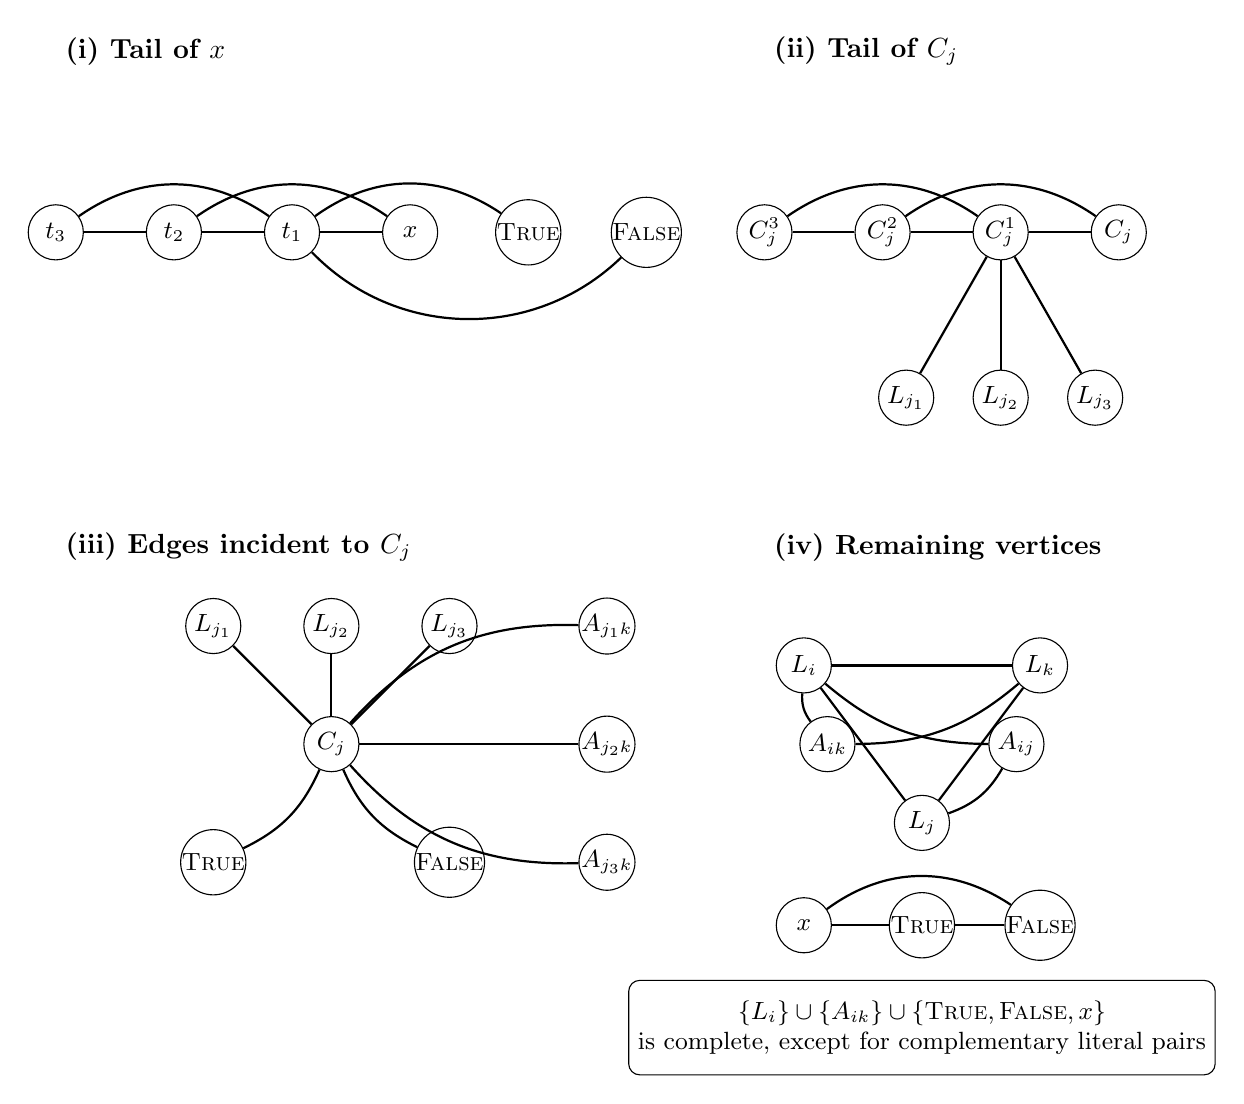
\begin{tikzpicture}[
    vertex/.style={
        circle,
        draw,
        fill=white,
        minimum size=7mm,
        inner sep=0pt,
        font=\small
    },
    edge/.style={thick},
    every node/.style={font=\small}
]

\begin{scope}[xshift=0cm,yshift=0cm]

\node[anchor=west,font=\bfseries] at (0,4.8)
    {(i) Tail of $x$};

\node[vertex] (t3) at (0,2.5) {$t_3$};
\node[vertex] (t2) at (1.5,2.5) {$t_2$};
\node[vertex] (t1) at (3.0,2.5) {$t_1$};
\node[vertex] (x)  at (4.5,2.5) {$x$};
\node[vertex] (T)  at (6.0,2.5) {$\textsc{True}$};
\node[vertex] (F)  at (7.5,2.5) {$\textsc{False}$};

\draw[edge] (t3)--(t2);
\draw[edge] (t2)--(t1);
\draw[edge] (t1)--(x);
\draw[edge] (t1) to[bend left=35] (T);
\draw[edge] (t3) to[bend left=35] (t1);
\draw[edge] (t2) to[bend left=35] (x);
\draw[edge] (t1) to[bend right=45] (F);

\end{scope}

\begin{scope}[xshift=9cm,yshift=0cm]

\node[anchor=west,font=\bfseries] at (0,4.8)
    {(ii) Tail of $C_j$};

\node[vertex] (c3) at (0,2.5) {$C_j^3$};
\node[vertex] (c2) at (1.5,2.5) {$C_j^2$};
\node[vertex] (c1) at (3.0,2.5) {$C_j^1$};
\node[vertex] (C)  at (4.5,2.5) {$C_j$};

\node[vertex] (L1) at (1.8,0.4) {$L_{j_1}$};
\node[vertex] (L2) at (3.0,0.4) {$L_{j_2}$};
\node[vertex] (L3) at (4.2,0.4) {$L_{j_3}$};

\draw[edge] (c3)--(c2);
\draw[edge] (c2)--(c1);
\draw[edge] (c1)--(C);

\draw[edge] (c3) to[bend left=35] (c1);
\draw[edge] (c2) to[bend left=35] (C);

\draw[edge] (c1)--(L1);
\draw[edge] (c1)--(L2);
\draw[edge] (c1)--(L3);

\end{scope}

\begin{scope}[xshift=0cm,yshift=-6.5cm]

\node[anchor=west,font=\bfseries] at (0,5.0)
    {(iii) Edges incident to $C_j$};

\node[vertex] (Cc) at (3.5,2.5) {$C_j$};

\node[vertex] (CL1) at (2.0,4.0) {$L_{j_1}$};
\node[vertex] (CL2) at (3.5,4.0) {$L_{j_2}$};
\node[vertex] (CL3) at (5.0,4.0) {$L_{j_3}$};

\node[vertex] (Tc) at (2.0,1.0) {$\textsc{True}$};
\node[vertex] (Fc) at (5.0,1.0) {$\textsc{False}$};

\node[vertex] (A1) at (7.0,4.0) {$A_{j_1k}$};
\node[vertex] (A2) at (7.0,2.5) {$A_{j_2k}$};
\node[vertex] (A3) at (7.0,1.0) {$A_{j_3k}$};

\draw[edge] (Cc)--(CL1);
\draw[edge] (Cc)--(CL2);
\draw[edge] (Cc)--(CL3);

\draw[edge] (Cc) to[bend left=20] (Tc);
\draw[edge] (Cc) to[bend right=20] (Fc);

\draw[edge] (Cc) to[bend left=25] (A1);
\draw[edge] (Cc)--(A2);
\draw[edge] (Cc) to[bend right=25] (A3);

\end{scope}

\begin{scope}[xshift=9cm,yshift=-6.5cm]

\node[anchor=west,font=\bfseries] at (0,5.0)
    {(iv) Remaining vertices};

\node[vertex] (Li) at (0.5,3.5) {$L_i$};
\node[vertex] (Lk) at (3.5,3.5) {$L_k$};
\node[vertex] (Lj) at (2.0,1.5) {$L_j$};

\node[vertex] (Aik) at (0.8,2.5) {$A_{ik}$};
\node[vertex] (Aij) at (3.2,2.5) {$A_{ij}$};

\node[vertex] (Dx) at (0.5,0.2) {$x$};
\node[vertex] (DT) at (2.0,0.2) {$\textsc{True}$};
\node[vertex] (DF) at (3.5,0.2) {$\textsc{False}$};

\draw[edge] (Li)--(Lk);
\draw[edge] (Li)--(Lj);
\draw[edge] (Lk)--(Lj);

\draw[edge] (Aik) to[bend left=20] (Li);
\draw[edge] (Aik) to[bend right=20] (Lk);

\draw[edge] (Aij) to[bend left=20] (Li);
\draw[edge] (Aij) to[bend left=20] (Lj);

\draw[edge] (Dx)--(DT);
\draw[edge] (Dx) to[bend left=35] (DF);
\draw[edge] (DT)--(DF);

\node[draw,rounded corners,align=center,
      minimum width=6.5cm,minimum height=1.2cm]
      at (2.0,-1.1)
      {$\{L_i\}\cup\{A_{ik}\}\cup
        \{\textsc{True},\textsc{False},x\}$\\
       is complete, except for complementary literal pairs};

\end{scope}
\end{tikzpicture}
\label{fig:polynomial-reduction}
\end{figure}
